\section[Background]{Background}

\begin{frame}{Reconstructing Dynamics from Snapshots}

\centering
We are interested in studying {\bf developmental dynamics}

\def\figwidth{0.1\textwidth}

\only<1>{
\begin{tikzpicture}
\node[draw=red] (fig1) {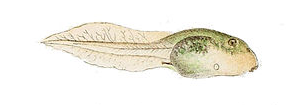
\includegraphics[width=\figwidth]{frog1}};
\node[draw=red,right=of fig1] (fig2) {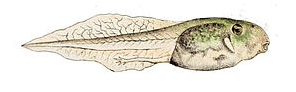
\includegraphics[width=\figwidth]{frog2}};
\node[draw=red,right=of fig2] (fig3) {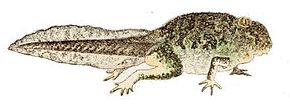
\includegraphics[width=\figwidth]{frog3}};
\node[draw=red,right=of fig3] (fig4) {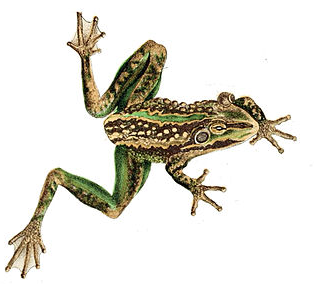
\includegraphics[width=\figwidth]{frog4}};
\draw[->] (fig1) -- (fig2);
\draw[->] (fig2) -- (fig3);
\draw[->] (fig3) -- (fig4);
\node[left=of fig1]{Sample};
\end{tikzpicture}}

\only<2>{
\begin{tikzpicture}
\node[] (fig1) {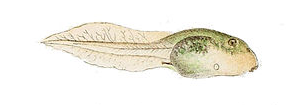
\includegraphics[width=\figwidth]{frog1}};
\node[draw=red,right=of fig1] (fig2) {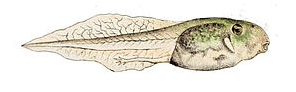
\includegraphics[width=\figwidth]{frog2}};
\node[right=of fig2] (fig3) {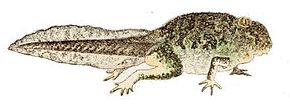
\includegraphics[width=\figwidth]{frog3}};
\node[right=of fig3] (fig4) {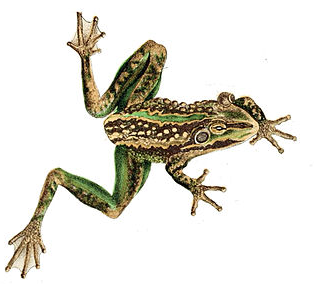
\includegraphics[width=\figwidth]{frog4}};
\draw[->] (fig1) -- (fig2);
\draw[->] (fig2) -- (fig3);
\draw[->] (fig3) -- (fig4);
\node[left=of fig1]{Sample 1};
\end{tikzpicture}}

\pause

\begin{tikzpicture}
\node (fig1) {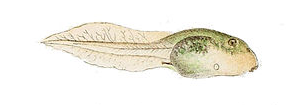
\includegraphics[width=\figwidth]{frog1}};
\node[right=of fig1] (fig2) {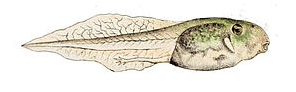
\includegraphics[width=\figwidth]{frog2}};
\node[draw=red,right=of fig2] (fig3) {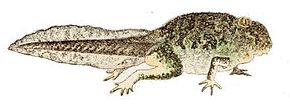
\includegraphics[width=\figwidth]{frog3}};
\node[right=of fig3] (fig4) {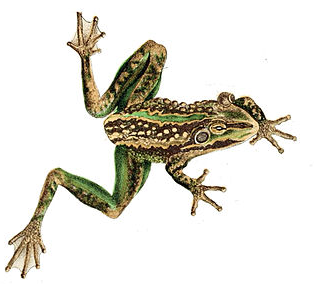
\includegraphics[width=\figwidth]{frog4}};
\draw[->] (fig1) -- (fig2);
\draw[->] (fig2) -- (fig3);
\draw[->] (fig3) -- (fig4);
\node[left=of fig1]{Sample 2};
\end{tikzpicture}

\begin{tikzpicture}
\node[draw=red] (fig1) {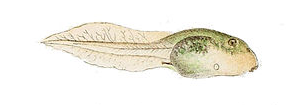
\includegraphics[width=\figwidth]{frog1}};
\node[right=of fig1] (fig2) {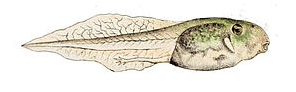
\includegraphics[width=\figwidth]{frog2}};
\node[right=of fig2] (fig3) {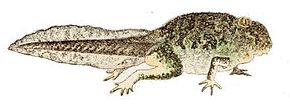
\includegraphics[width=\figwidth]{frog3}};
\node[right=of fig3] (fig4) {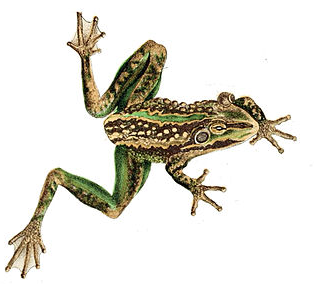
\includegraphics[width=\figwidth]{frog4}};
\draw[->] (fig1) -- (fig2);
\draw[->] (fig2) -- (fig3);
\draw[->] (fig3) -- (fig4);
\node[left=of fig1]{Sample 3};
\end{tikzpicture}

\begin{tikzpicture}
\node (fig1) {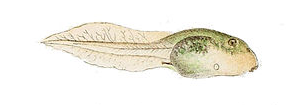
\includegraphics[width=\figwidth]{frog1}};
\node[right=of fig1] (fig2) {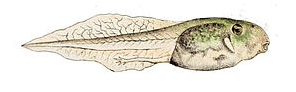
\includegraphics[width=\figwidth]{frog2}};
\node[right=of fig2] (fig3) {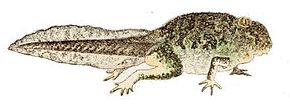
\includegraphics[width=\figwidth]{frog3}};
\node[draw=red,right=of fig3] (fig4) {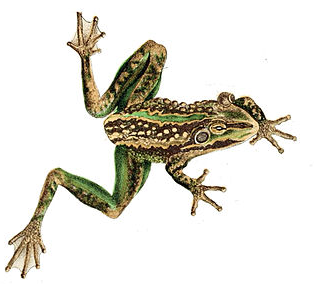
\includegraphics[width=\figwidth]{frog4}};
\draw[->] (fig1) -- (fig2);
\draw[->] (fig2) -- (fig3);
\draw[->] (fig3) -- (fig4);
\node[left=of fig1]{Sample 4};
\end{tikzpicture}

{\small
\begin{itemize}
\item We cannot obtain one continuous trajectory from one organism ({\bf longitudinal~data}).
%
\item Instead, we have one snapshot from the developmental trajectory of each organism ({\bf cross--sectional data})
%
\item We need a way to {\em order} the snapshots  to reconstruct the developmental dynamics.
\end{itemize}
}
\end{frame}

\begin{frame}{Dynamics of ERK Activation in {\em Drosophila}}
	
	\centering
	We would like to reconstruct the spatiotemporal dynamics \\
	of the activation of the ERK pathway in {\em Drosophila} embryos\\
	during nuclear cycle 14 (the third hour of development)

    \centering
	\begin{minipage}{0.3\textwidth}
	    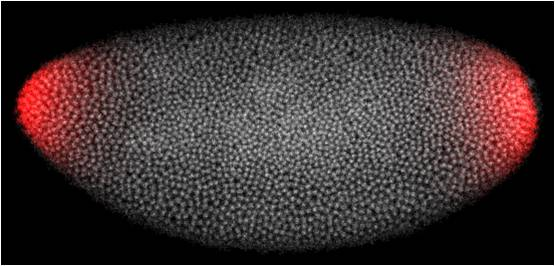
\includegraphics[width=\textwidth]{erk_10min}\\
	    {\scriptsize \em 10 minutes \par}
	\end{minipage}
	\begin{minipage}{0.3\textwidth}
	    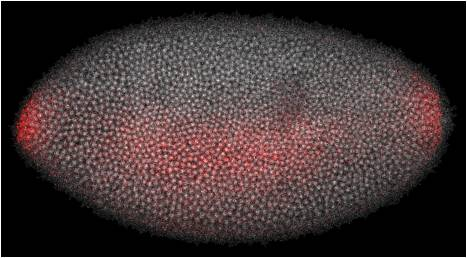
\includegraphics[width=\textwidth]{erk_25min}\\
	    {\scriptsize \em 25 minutes \par}
	\end{minipage}
	\begin{minipage}{0.3\textwidth}
	    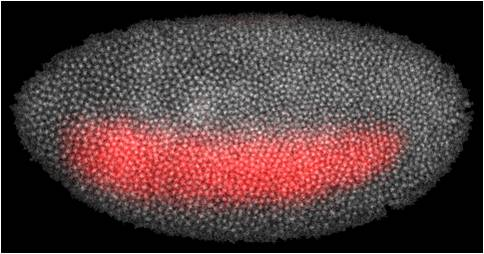
\includegraphics[width=\textwidth]{erk_45min}\\
	    {\scriptsize \em 45 minutes \par}
	\end{minipage}
	
	{\small {\em Drosophila} embryos stained for dpERK}
	
	\begin{itemize}
		\item We measure the activation of ERK by staining embryos for double-phosphorylated ERK (dpERK); ERK is double-phosphorylated  directly downstream of the ERK pathway, and so the presence of dpERK indicates activation of the ERK pathway
	
		\item However, we cannot fluorescently tag ERK within the developing embryo because we are interested in a specific phosphorylation state of the molecule
		
		\item Instead, we must {\em fix} the embryo and then use an antibody stain for dpERK
	
		\item Therefore, we cannot obtain live images of the evolution of dpERK in {\em Drosophila} embryos
	\end{itemize}
	
\end{frame}

\begin{frame}{Imaging Dorsoventral Patterns in {\em Drosophila} \footcite{chung2010microfluidic}}

	\centering
    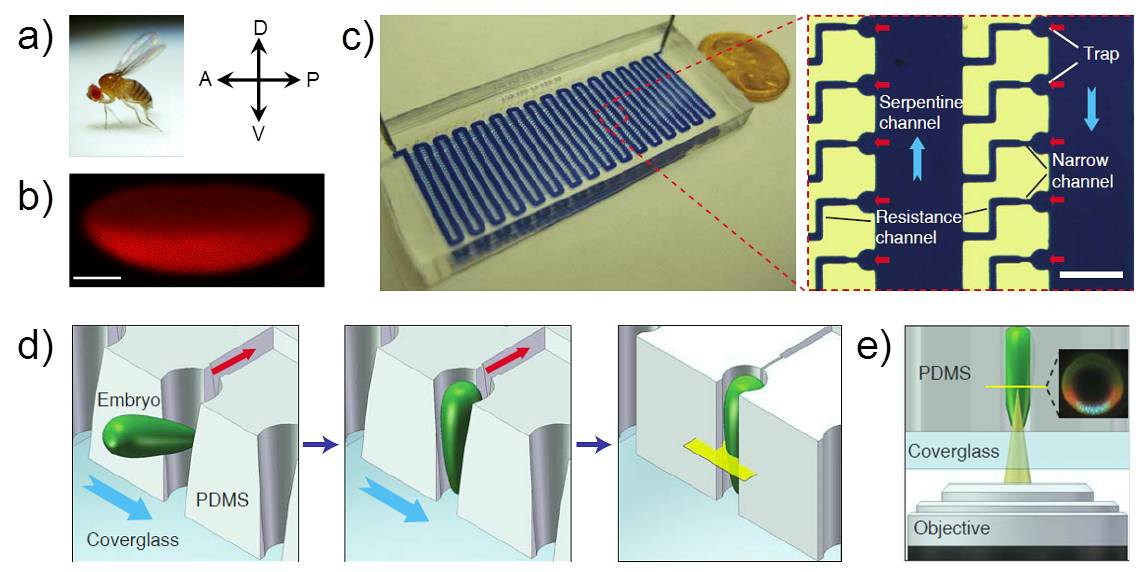
\includegraphics[width=0.75\textwidth]{drosophila_imaging_setup}
    
	\begin{itemize}
        \item We can easily obtain snapshots of many {\em Drosophila} embryos using a high--throughput microfluidic device
        \item Each embryo is fixed at a slightly different developmental time (``cross-sectional data'')
        \item We would like to temporally order the data from multiple embryos to~reconstruct the developmental dynamics in {\em Drosophila}
    \end{itemize}
\end{frame}


\begin{frame}{Fluorescent {\em Drosophila} Images}
	 
	\drawunordered
	
	\drawdownarrow
	
	\drawordereddmaps
	
	We will discuss how to use data mining techniques to order the raw images so~that we can easily see the developmental dynamics.

\end{frame}

\begin{frame}{Reconstructing Dynamics from Snapshots}

	\begin{tikzpicture}
		\node (schematic) {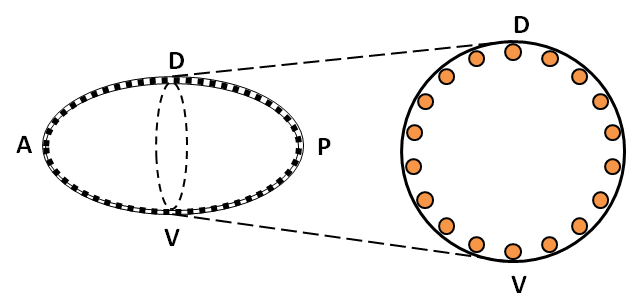
\includegraphics[width=0.25\textwidth]{drosophila_schematic}};
		\node [below=0in of schematic, text width=0.2\textwidth, align=center] (text1) {{\scriptsize Schematic of {\em Drosophila} embryo \\ (longitudinal and cross-section) \par}};

		\node [right=0.2in of schematic] (dpERK_image) {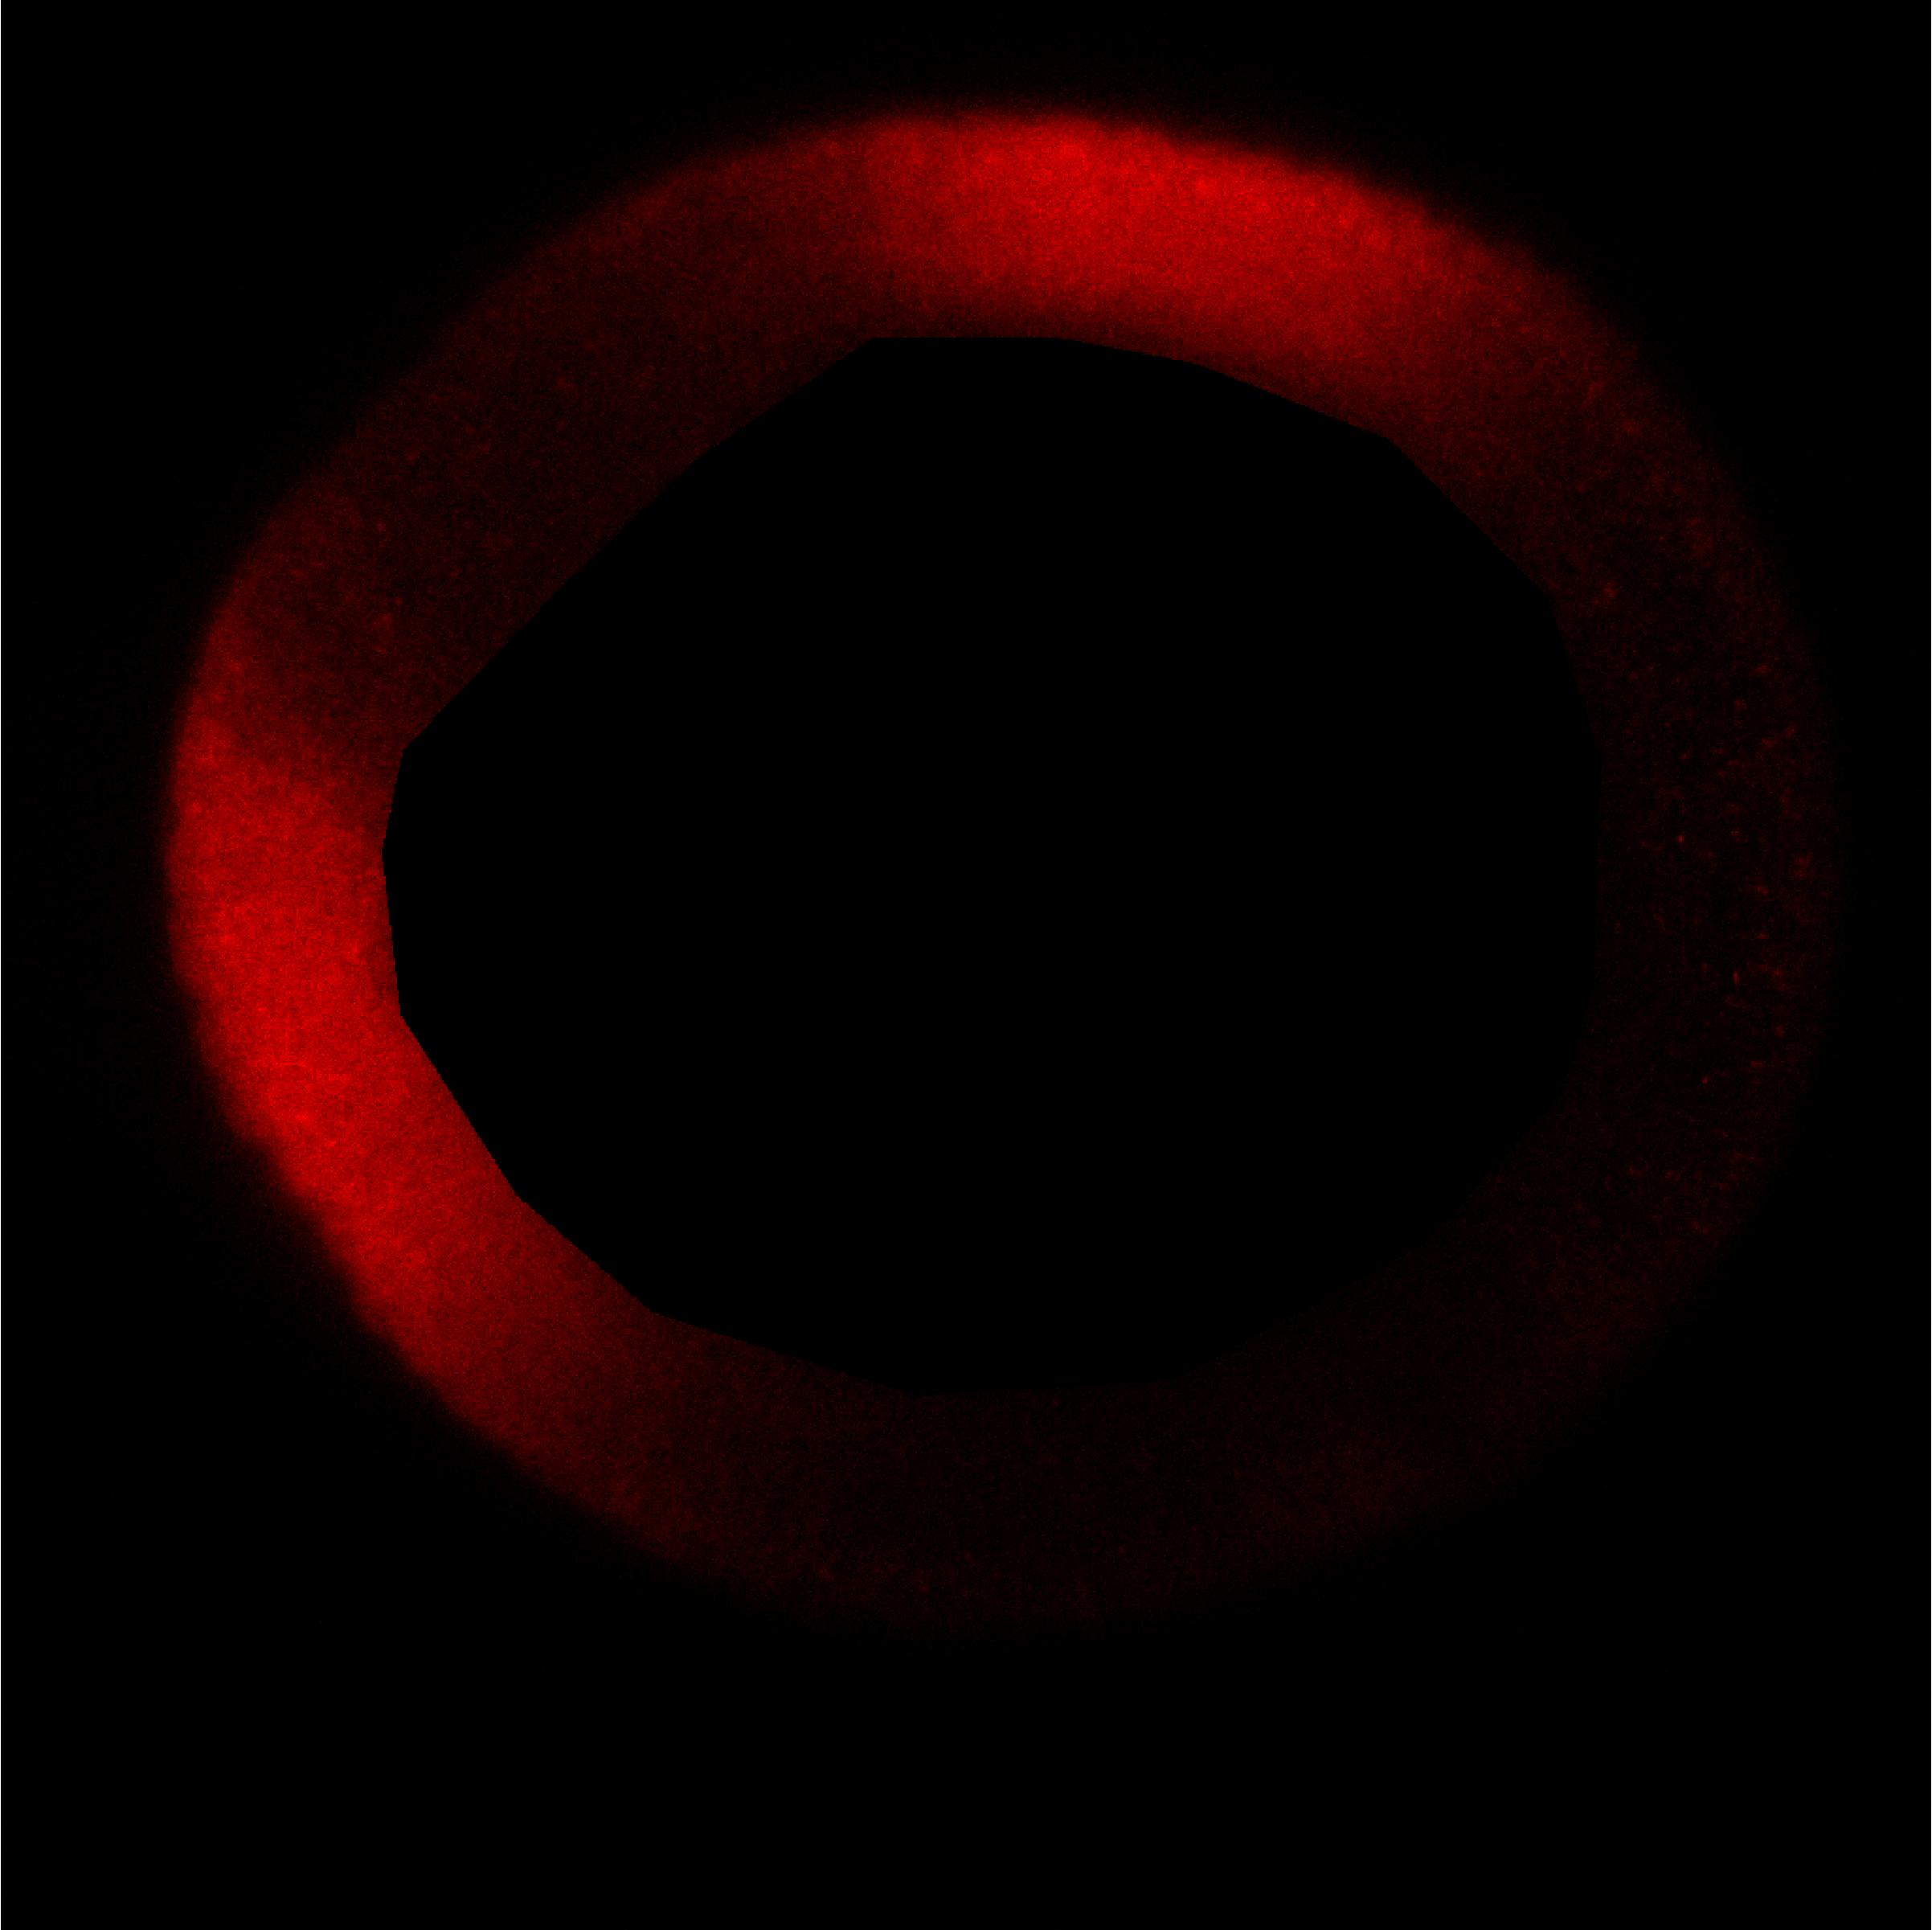
\includegraphics[width=0.15\textwidth]{drosophila_dpERK}} edge[<-] (schematic);
		\draw[gray,<->] (dpERK_image.south west) --  (dpERK_image.south east) node[below,midway] { \tiny $100 \mu m$};
		\node [below=0.1in of dpERK_image, text width=0.2\textwidth, align=center] (text1) {{\scriptsize Embryo cross-section fluorescently stained for the protein dpERK \par}};
		
		\node [right=0.2in of dpERK_image] (dpERK_circle) {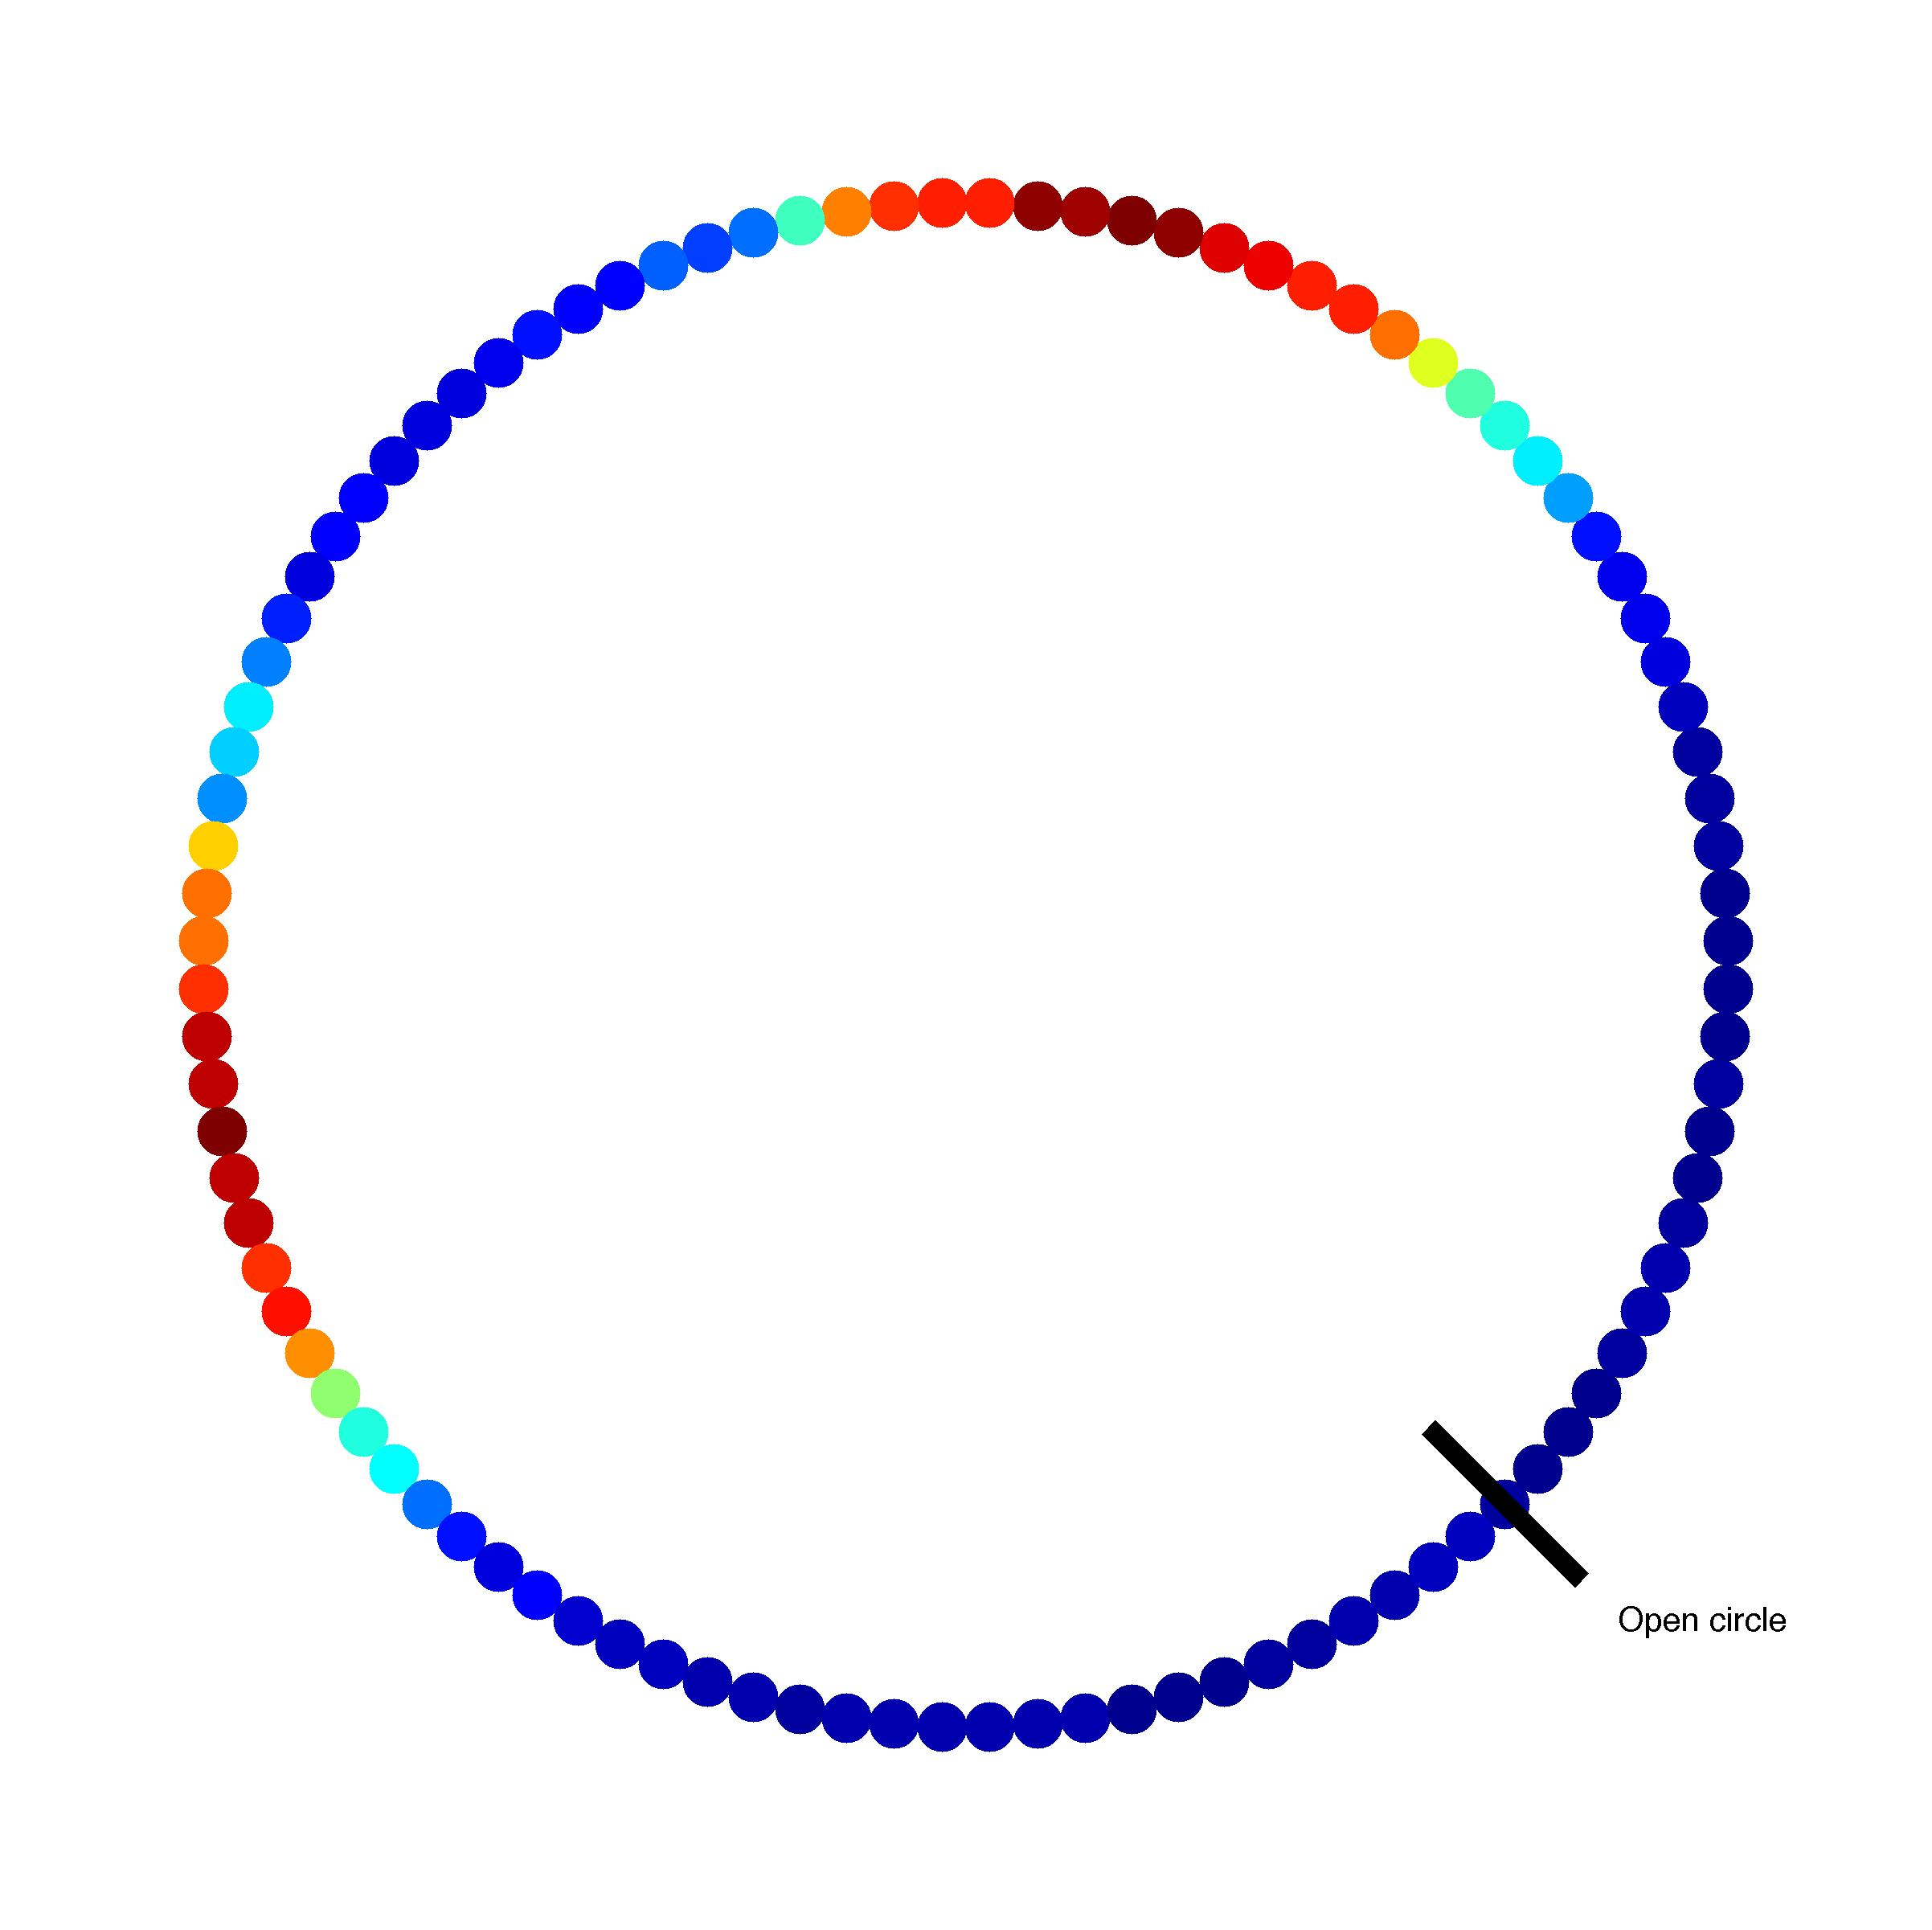
\includegraphics[width=0.15\textwidth]{circle_profile.jpg}} edge[<-] (dpERK_image);
		\node [below=0in of dpERK_circle, text width=0.2\textwidth, align=center] (text1) {{\scriptsize Fluorescent staining is converted to intensity of dpERK around the circumference of the embryo \par}};
		
		\node [right=0.2in of dpERK_circle] (dpERK_line) {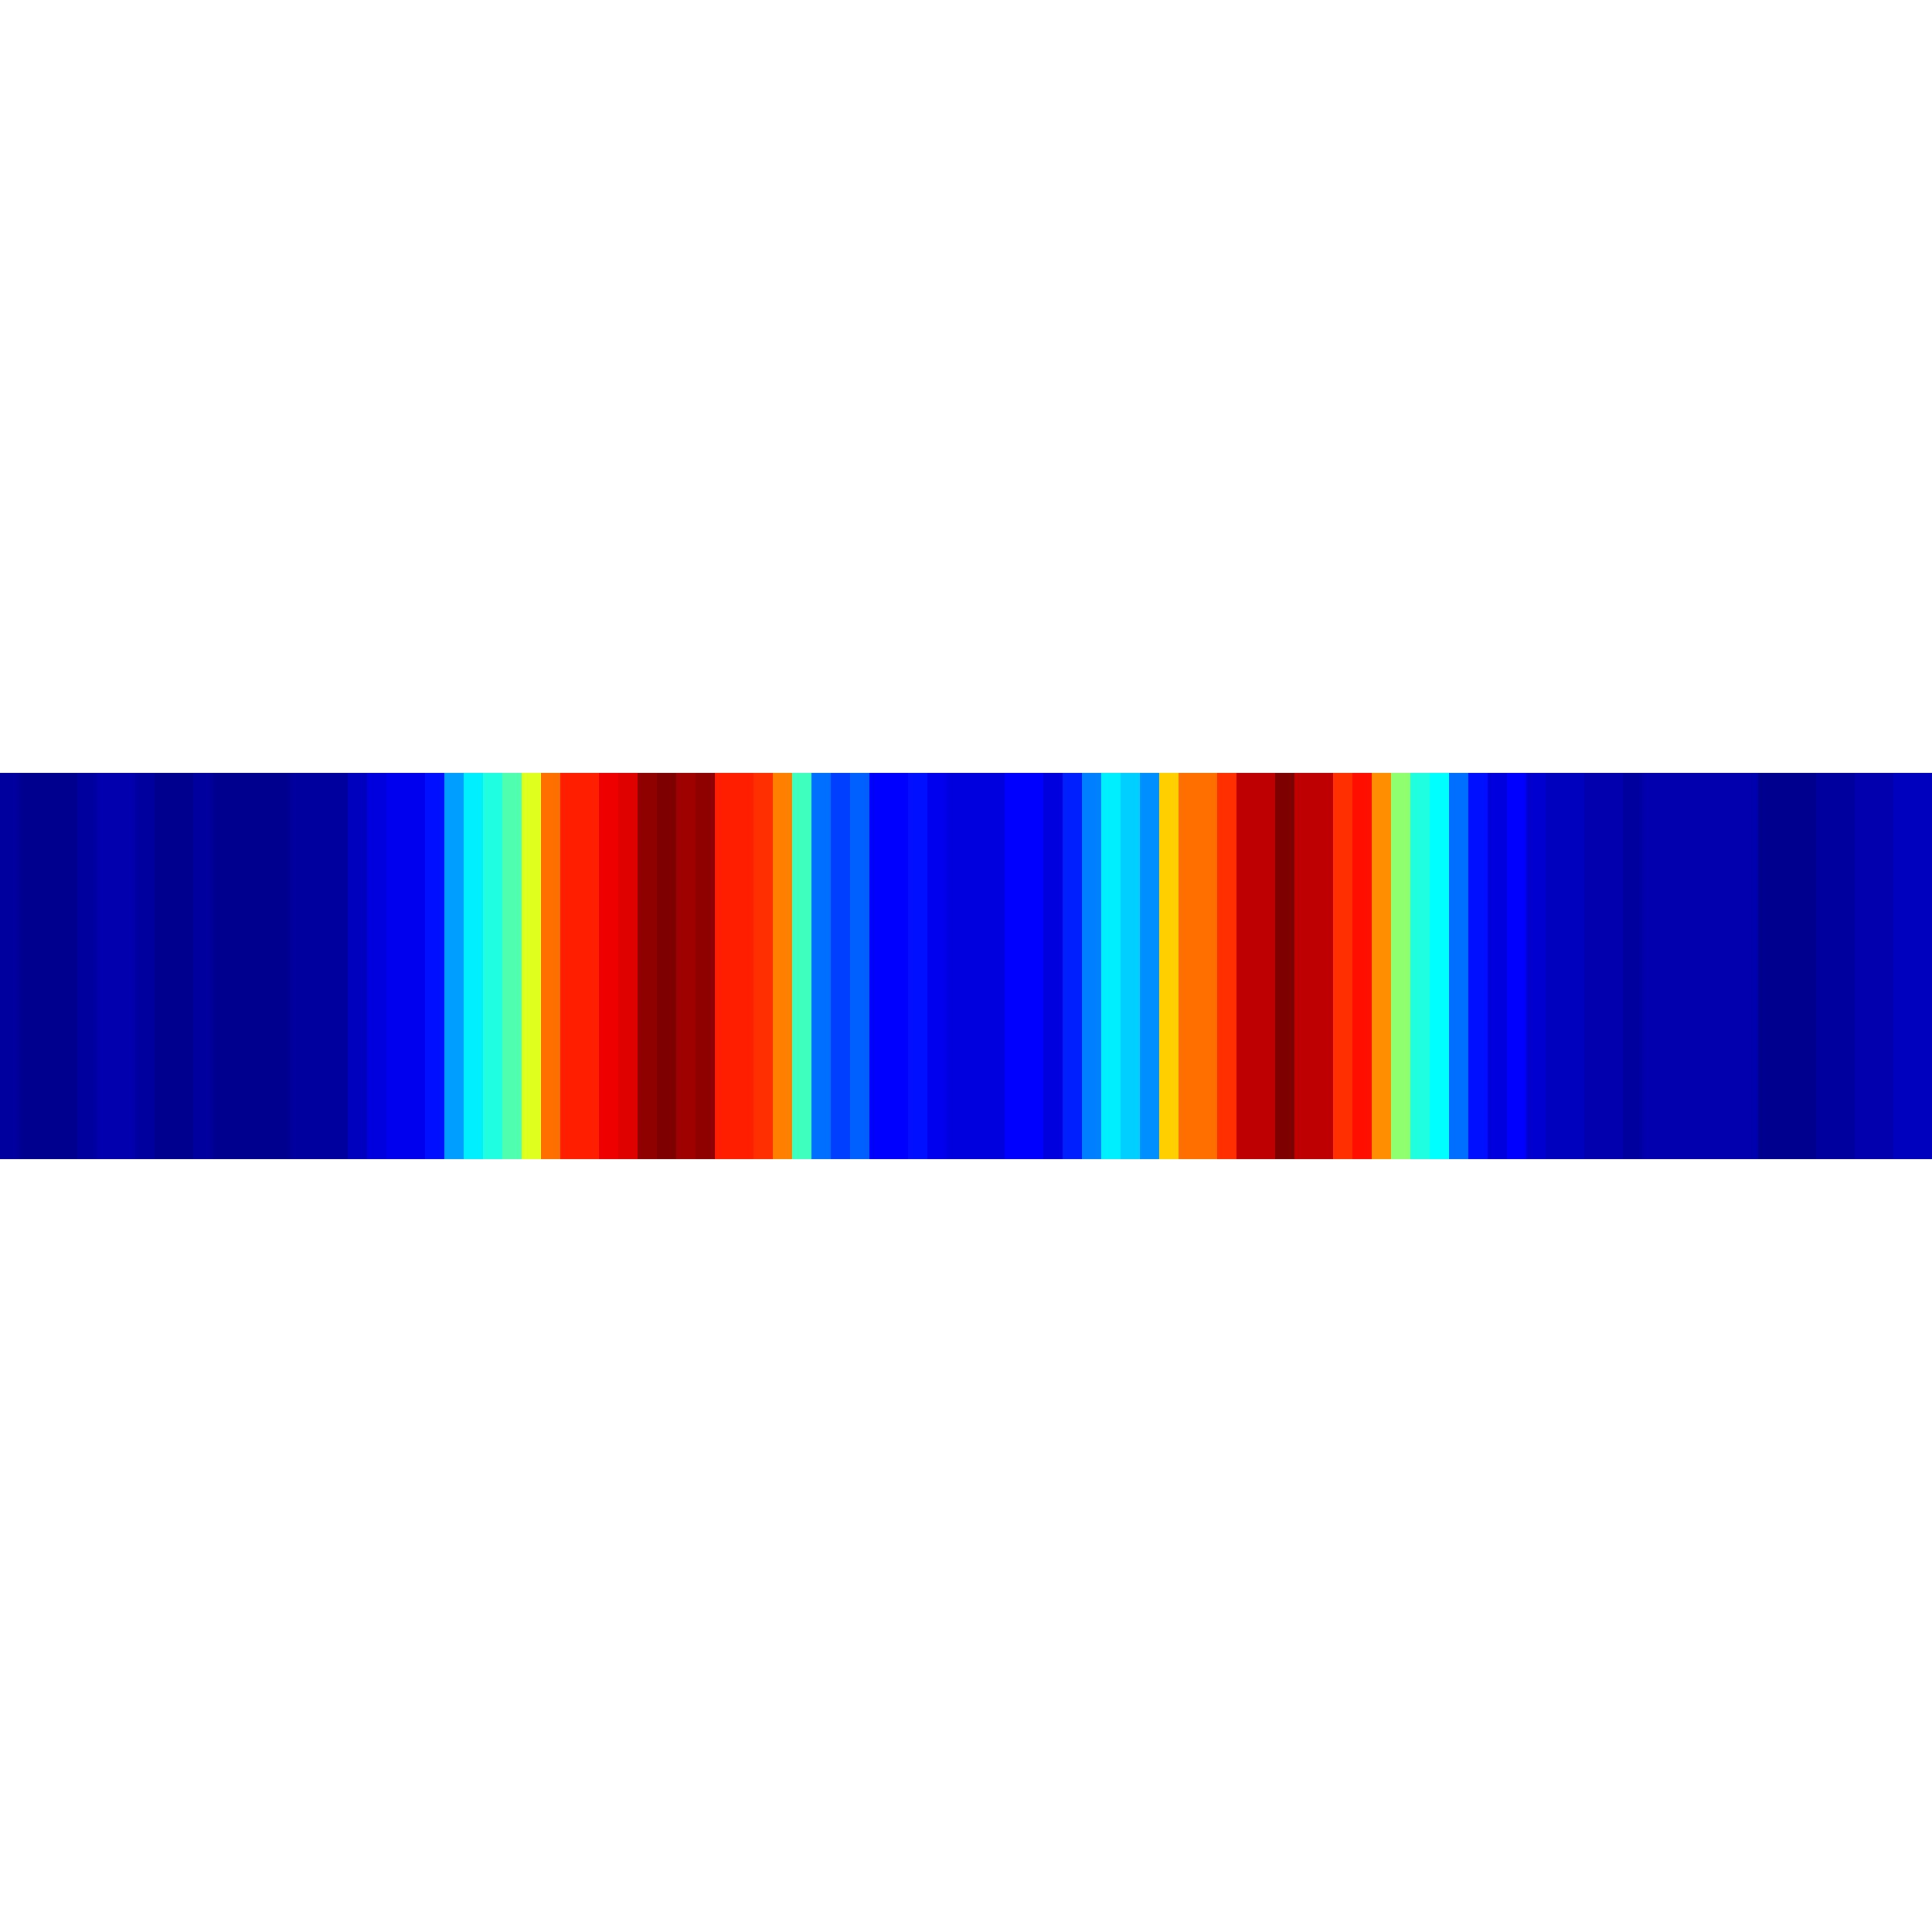
\includegraphics[width=0.2\textwidth, height=0.1in]{line_profile.jpg}} edge[<-] (dpERK_circle);
		\node [below=0in of dpERK_line, text width=0.2\textwidth, align=center] (text1) {{\scriptsize The circumference of the embryo is ``unrolled'' to form an intensity profile for the embryo on a line \par}};
		
	\end{tikzpicture}
	
	\centering
    \begin{tikzpicture}
        \node (fig1) {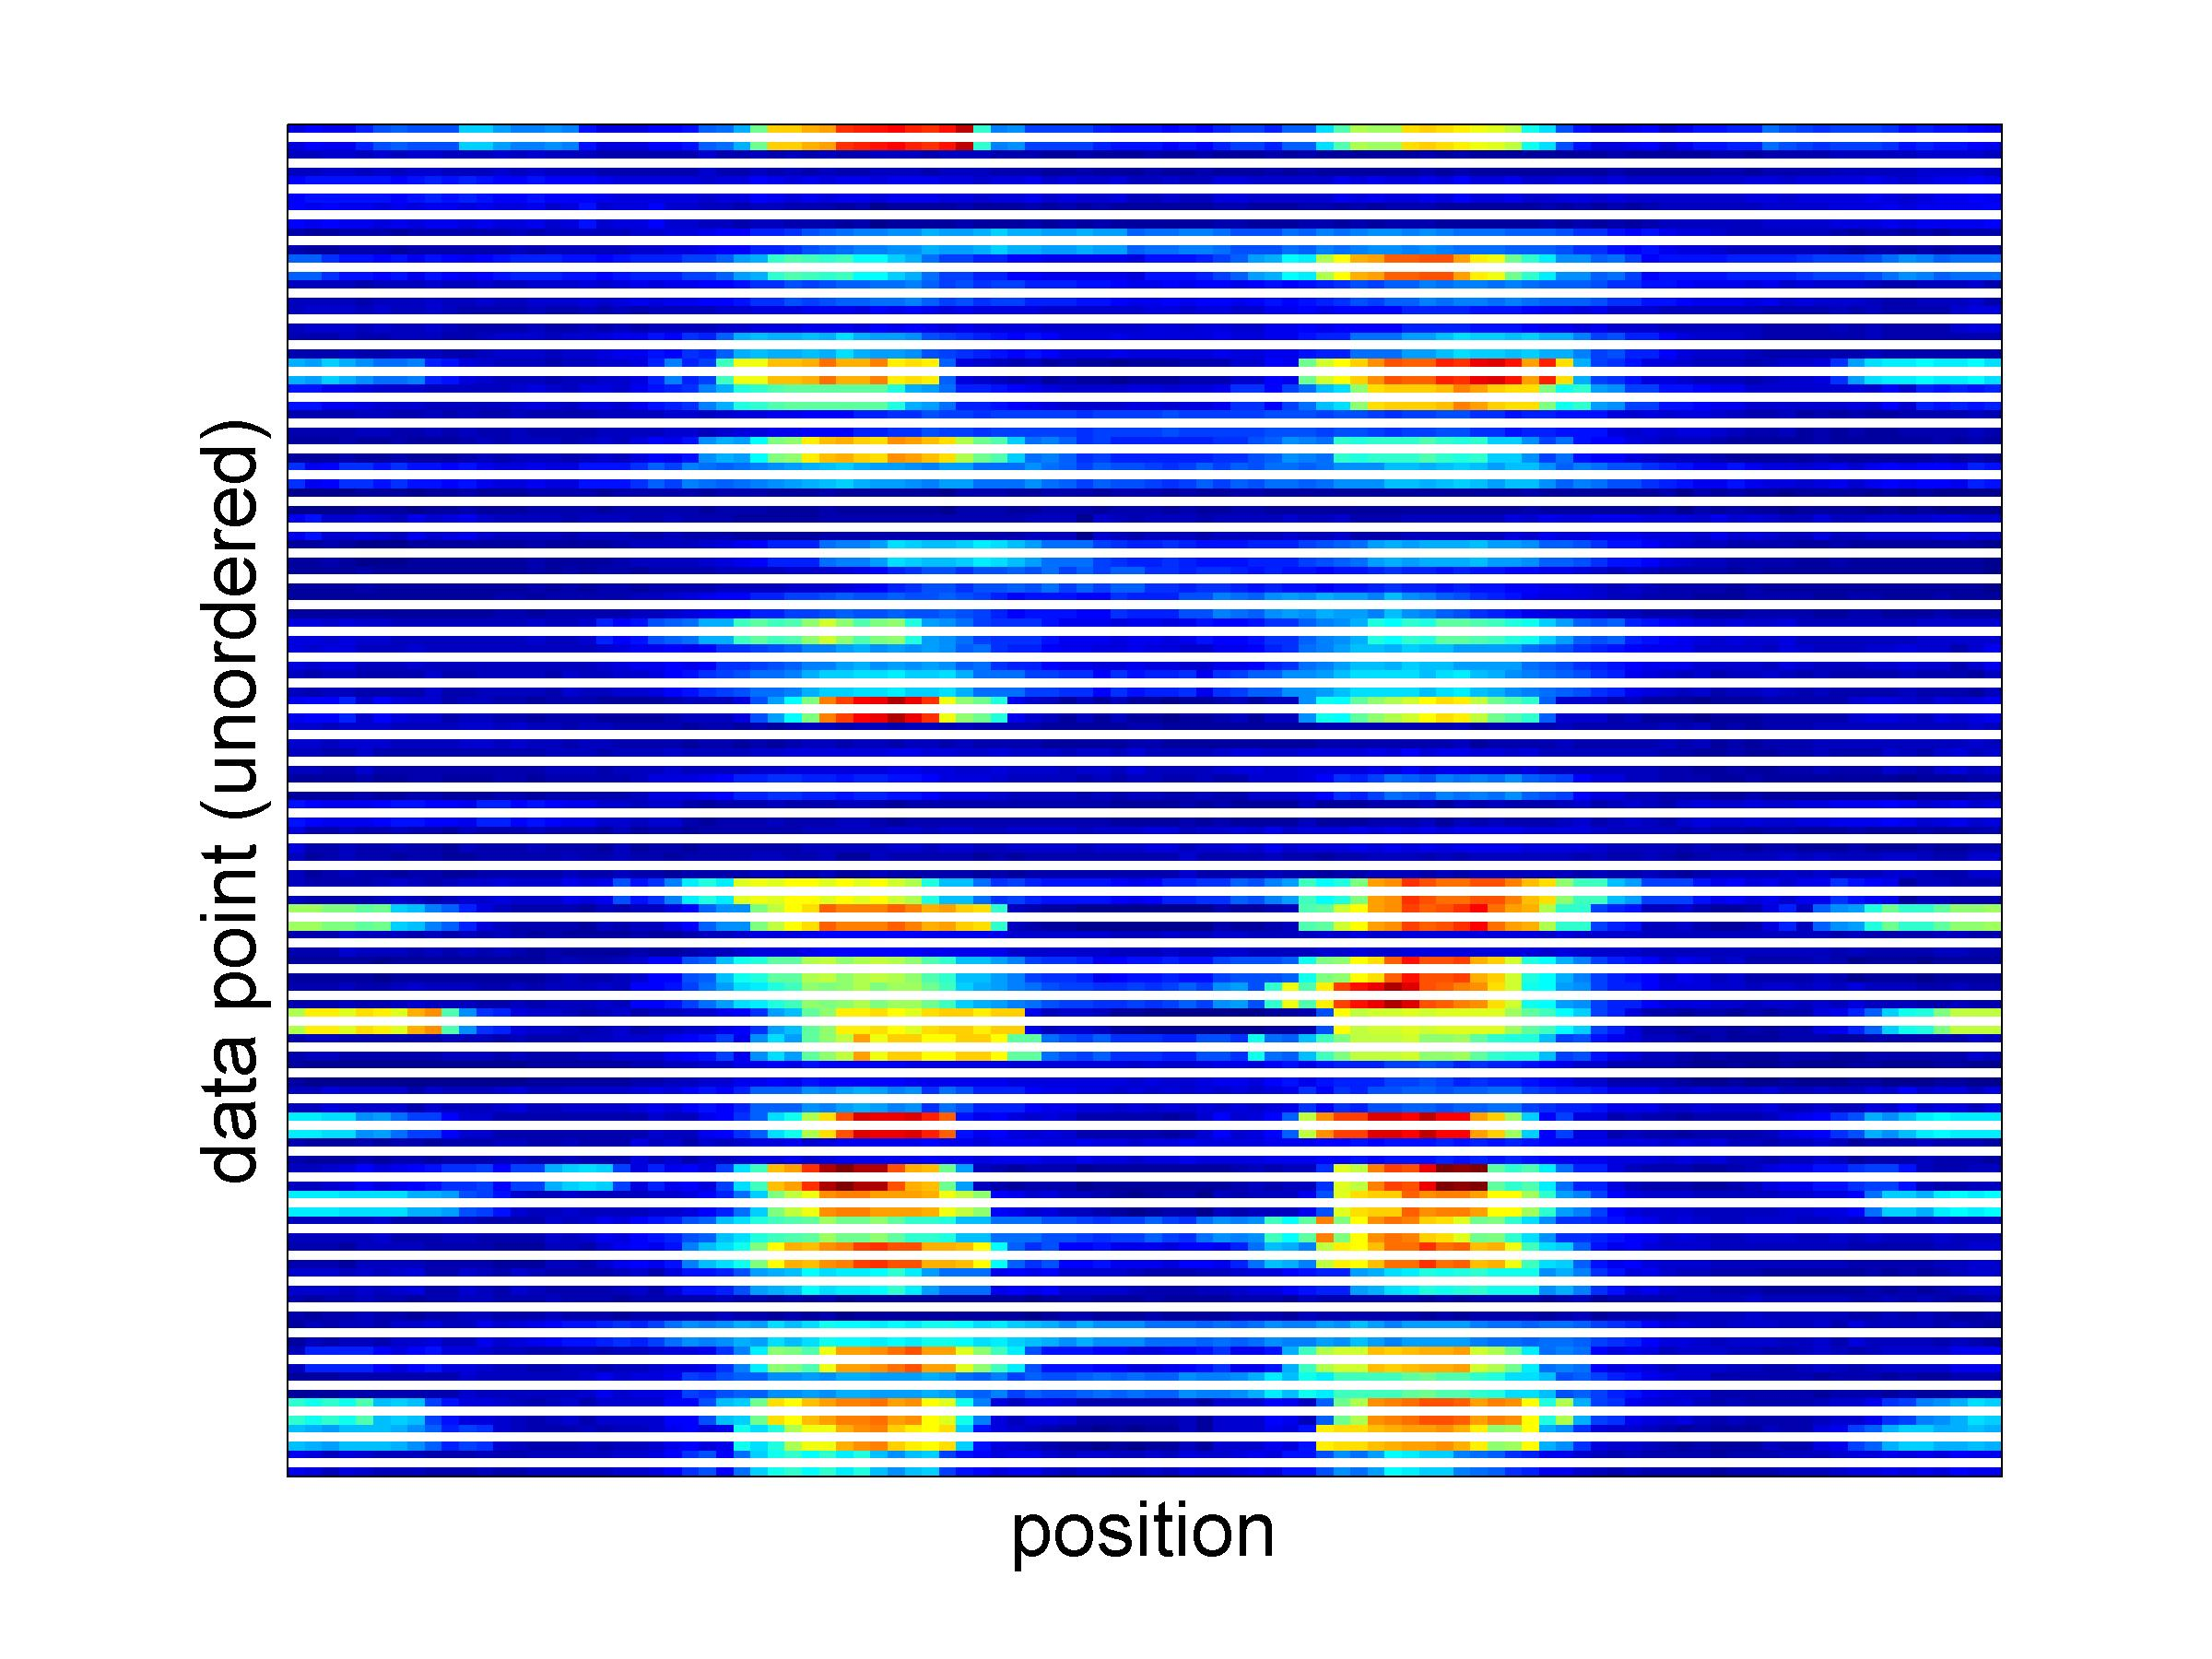
\includegraphics[width=0.3\textwidth]{data_unordered_spaced}};
        \node[right of=fig1, node distance=0.55\textwidth] (fig2) {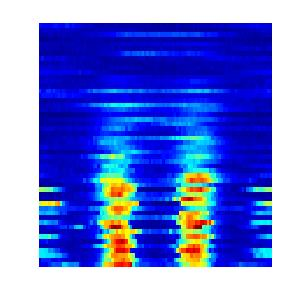
\includegraphics[width=0.3\textwidth]{data_ordered_membrane}};
        \draw [->] (fig1.east) -- (fig2.west) node[above,midway] {\tiny Order temporally};
    \end{tikzpicture}
	
	We will discuss how we can do each of these steps in the data analysis pipeline {\em automatically} using data mining techniques. 
	
\end{frame}
